\documentclass[tikz,border=0mm]{standalone}
\usepackage[utf8]{inputenc}
\usepackage{unicode-math} % for unicode support in math environments
\usepackage{amsmath}
\usepackage{siunitx}
\usepackage{booktabs}
\sisetup{mode=text,range-phrase = {\text{~to~}}, range-units=single, print-unity-mantissa=false}
\usepackage{mhchem}
\usepackage{tikz}



\usepackage{fontspec}

\directlua{
  luaotfload.add_fallback(
  "FallbackFonts",
  {
        "DejaVu Serif:mode=harf;",
        "DejaVu Sans Mono:mode=harf;",
        % we could add many more fonts here optionally!
    }
  )
}

\setmainfont{CMU Serif}[RawFeature={fallback=FallbackFonts}]
\setmonofont{Inconsolata}[RawFeature={fallback=FallbackFonts}]

\begin{document}
\definecolor{backgroundColor}{rgb}{1.0, 1.0, 1.0}

\pagecolor{backgroundColor}


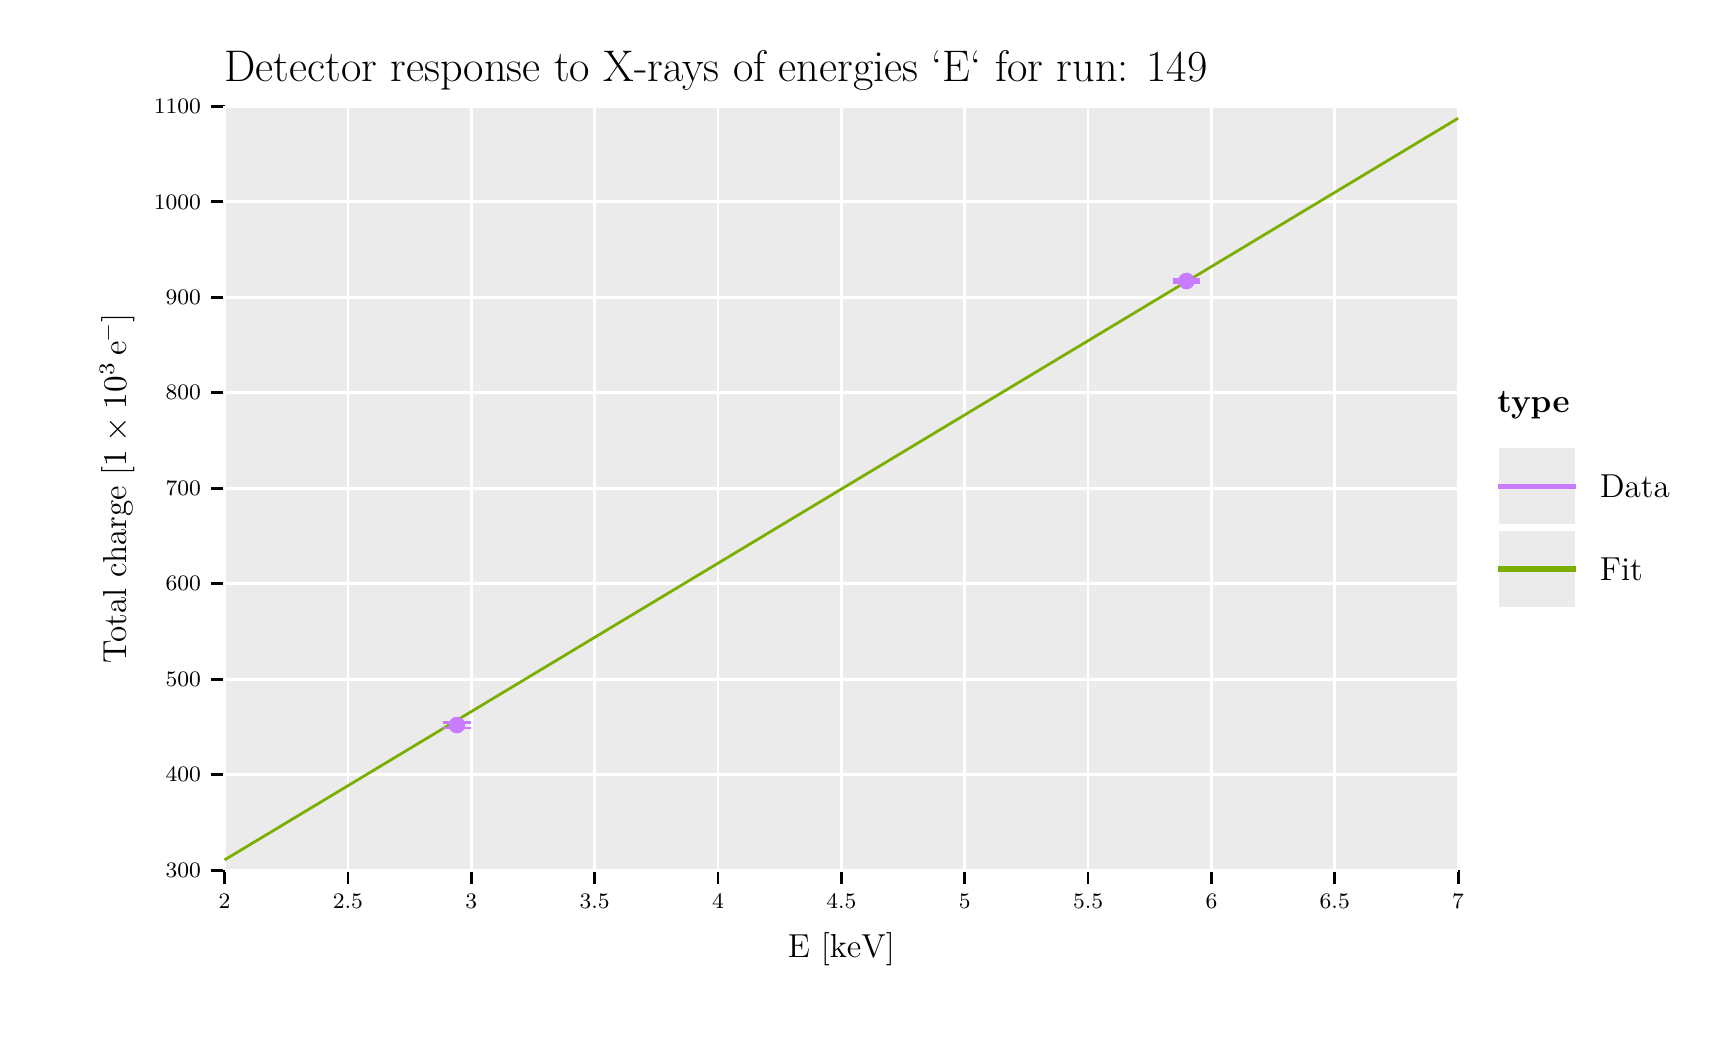
\begin{tikzpicture}[every node/.style={outer sep=0pt, inner sep=0pt}]
\path[use as bounding box] (0, 0) rectangle (600.0bp, 360.0bp) ;
\definecolor{drawColor}{rgb}{0.0, 0.0, 0.0}
\definecolor{fillColor}{rgb}{1.0, 1.0, 1.0}

\draw [color = drawColor, fill = fillColor, draw opacity = 0.0, fill opacity = 1.0, line width = 0.0bp] (0.0000bp, 360.0000bp) rectangle (600.0000bp, 0.0000bp) ;
\node [right, font=\fontsize{16.0}{19.2}\selectfont
, anchor=west] at (70.8661bp, 344.4711bp){Detector response to X-rays of energies `E` for run: 149} ;
\definecolor{drawColor}{rgb}{0.0, 0.0, 0.0}
\definecolor{fillColor}{rgb}{0.9200000166893005, 0.9200000166893005, 0.9200000166893005}

\draw [color = drawColor, fill = fillColor, draw opacity = 0.0, fill opacity = 1.0, line width = 0.0bp] (70.8661bp, 331.6535bp) rectangle (514.9606bp, 56.6929bp) ;
\definecolor{drawColor}{rgb}{0.0, 0.0, 0.0}
\definecolor{fillColor}{rgb}{0.0, 0.0, 0.0}

\draw [color = drawColor, fill = fillColor, draw opacity = 1.0, fill opacity = 0.0, line width = 1.0bp] (70.8661bp, 51.6929bp)--(70.8661bp, 56.6929bp) ;
\draw [color = drawColor, fill = fillColor, draw opacity = 1.0, fill opacity = 0.0, line width = 1.0bp] (115.2756bp, 51.6929bp)--(115.2756bp, 56.6929bp) ;
\draw [color = drawColor, fill = fillColor, draw opacity = 1.0, fill opacity = 0.0, line width = 1.0bp] (159.6850bp, 51.6929bp)--(159.6850bp, 56.6929bp) ;
\draw [color = drawColor, fill = fillColor, draw opacity = 1.0, fill opacity = 0.0, line width = 1.0bp] (204.0945bp, 51.6929bp)--(204.0945bp, 56.6929bp) ;
\draw [color = drawColor, fill = fillColor, draw opacity = 1.0, fill opacity = 0.0, line width = 1.0bp] (248.5039bp, 51.6929bp)--(248.5039bp, 56.6929bp) ;
\draw [color = drawColor, fill = fillColor, draw opacity = 1.0, fill opacity = 0.0, line width = 1.0bp] (292.9134bp, 51.6929bp)--(292.9134bp, 56.6929bp) ;
\draw [color = drawColor, fill = fillColor, draw opacity = 1.0, fill opacity = 0.0, line width = 1.0bp] (337.3228bp, 51.6929bp)--(337.3228bp, 56.6929bp) ;
\draw [color = drawColor, fill = fillColor, draw opacity = 1.0, fill opacity = 0.0, line width = 1.0bp] (381.7323bp, 51.6929bp)--(381.7323bp, 56.6929bp) ;
\draw [color = drawColor, fill = fillColor, draw opacity = 1.0, fill opacity = 0.0, line width = 1.0bp] (426.1417bp, 51.6929bp)--(426.1417bp, 56.6929bp) ;
\draw [color = drawColor, fill = fillColor, draw opacity = 1.0, fill opacity = 0.0, line width = 1.0bp] (470.5512bp, 51.6929bp)--(470.5512bp, 56.6929bp) ;
\draw [color = drawColor, fill = fillColor, draw opacity = 1.0, fill opacity = 0.0, line width = 1.0bp] (514.9606bp, 51.6929bp)--(514.9606bp, 56.6929bp) ;
\node [font=\fontsize{8.0}{9.6}\selectfont
] at (70.8661bp, 45.5272bp){2} ;
\node [font=\fontsize{8.0}{9.6}\selectfont
] at (115.2756bp, 45.4389bp){2.5} ;
\node [font=\fontsize{8.0}{9.6}\selectfont
] at (159.6850bp, 45.4389bp){3} ;
\node [font=\fontsize{8.0}{9.6}\selectfont
] at (204.0945bp, 45.4389bp){3.5} ;
\node [font=\fontsize{8.0}{9.6}\selectfont
] at (248.5039bp, 45.4830bp){4} ;
\node [font=\fontsize{8.0}{9.6}\selectfont
] at (292.9134bp, 45.3947bp){4.5} ;
\node [font=\fontsize{8.0}{9.6}\selectfont
] at (337.3228bp, 45.4389bp){5} ;
\node [font=\fontsize{8.0}{9.6}\selectfont
] at (381.7323bp, 45.4389bp){5.5} ;
\node [font=\fontsize{8.0}{9.6}\selectfont
] at (426.1417bp, 45.4389bp){6} ;
\node [font=\fontsize{8.0}{9.6}\selectfont
] at (470.5512bp, 45.4389bp){6.5} ;
\node [font=\fontsize{8.0}{9.6}\selectfont
] at (514.9606bp, 45.3987bp){7} ;
\draw [color = drawColor, fill = fillColor, draw opacity = 1.0, fill opacity = 0.0, line width = 1.0bp] (70.8661bp, 56.6929bp)--(65.8661bp, 56.6929bp) ;
\draw [color = drawColor, fill = fillColor, draw opacity = 1.0, fill opacity = 0.0, line width = 1.0bp] (70.8661bp, 91.0630bp)--(65.8661bp, 91.0630bp) ;
\draw [color = drawColor, fill = fillColor, draw opacity = 1.0, fill opacity = 0.0, line width = 1.0bp] (70.8661bp, 125.4331bp)--(65.8661bp, 125.4331bp) ;
\draw [color = drawColor, fill = fillColor, draw opacity = 1.0, fill opacity = 0.0, line width = 1.0bp] (70.8661bp, 159.8031bp)--(65.8661bp, 159.8031bp) ;
\draw [color = drawColor, fill = fillColor, draw opacity = 1.0, fill opacity = 0.0, line width = 1.0bp] (70.8661bp, 194.1732bp)--(65.8661bp, 194.1732bp) ;
\draw [color = drawColor, fill = fillColor, draw opacity = 1.0, fill opacity = 0.0, line width = 1.0bp] (70.8661bp, 228.5433bp)--(65.8661bp, 228.5433bp) ;
\draw [color = drawColor, fill = fillColor, draw opacity = 1.0, fill opacity = 0.0, line width = 1.0bp] (70.8661bp, 262.9134bp)--(65.8661bp, 262.9134bp) ;
\draw [color = drawColor, fill = fillColor, draw opacity = 1.0, fill opacity = 0.0, line width = 1.0bp] (70.8661bp, 297.2835bp)--(65.8661bp, 297.2835bp) ;
\draw [color = drawColor, fill = fillColor, draw opacity = 1.0, fill opacity = 0.0, line width = 1.0bp] (70.8661bp, 331.6535bp)--(65.8661bp, 331.6535bp) ;
\node [left, font=\fontsize{8.0}{9.6}\selectfont
, anchor=east] at (62.3744bp, 56.6929bp){300} ;
\node [left, font=\fontsize{8.0}{9.6}\selectfont
, anchor=east] at (62.3744bp, 91.0630bp){400} ;
\node [left, font=\fontsize{8.0}{9.6}\selectfont
, anchor=east] at (62.3744bp, 125.4331bp){500} ;
\node [left, font=\fontsize{8.0}{9.6}\selectfont
, anchor=east] at (62.3744bp, 159.8031bp){600} ;
\node [left, font=\fontsize{8.0}{9.6}\selectfont
, anchor=east] at (62.3744bp, 194.1732bp){700} ;
\node [left, font=\fontsize{8.0}{9.6}\selectfont
, anchor=east] at (62.3744bp, 228.5433bp){800} ;
\node [left, font=\fontsize{8.0}{9.6}\selectfont
, anchor=east] at (62.3744bp, 262.9134bp){900} ;
\node [left, font=\fontsize{8.0}{9.6}\selectfont
, anchor=east] at (62.3744bp, 297.2835bp){1000} ;
\node [left, font=\fontsize{8.0}{9.6}\selectfont
, anchor=east] at (62.3744bp, 331.6535bp){1100} ;
\node [font=\fontsize{12.0}{14.4}\selectfont
] at (292.9134bp, 28.3465bp){E [$\si{keV}$]} ;
\node [rotate = 90.0, font=\fontsize{12.0}{14.4}\selectfont
] at (32.1290bp, 194.1732bp){Total charge [$\SI{1e3}{e^-}$]} ;
\definecolor{drawColor}{rgb}{1.0, 1.0, 1.0}
\definecolor{fillColor}{rgb}{0.0, 0.0, 0.0}

\draw [color = drawColor, fill = fillColor, draw opacity = 1.0, fill opacity = 0.0, line width = 1.0bp] (70.8661bp, 331.6535bp)--(70.8661bp, 56.6929bp) ;
\draw [color = drawColor, fill = fillColor, draw opacity = 1.0, fill opacity = 0.0, line width = 1.0bp] (115.2756bp, 331.6535bp)--(115.2756bp, 56.6929bp) ;
\draw [color = drawColor, fill = fillColor, draw opacity = 1.0, fill opacity = 0.0, line width = 1.0bp] (159.6850bp, 331.6535bp)--(159.6850bp, 56.6929bp) ;
\draw [color = drawColor, fill = fillColor, draw opacity = 1.0, fill opacity = 0.0, line width = 1.0bp] (204.0945bp, 331.6535bp)--(204.0945bp, 56.6929bp) ;
\draw [color = drawColor, fill = fillColor, draw opacity = 1.0, fill opacity = 0.0, line width = 1.0bp] (248.5039bp, 331.6535bp)--(248.5039bp, 56.6929bp) ;
\draw [color = drawColor, fill = fillColor, draw opacity = 1.0, fill opacity = 0.0, line width = 1.0bp] (292.9134bp, 331.6535bp)--(292.9134bp, 56.6929bp) ;
\draw [color = drawColor, fill = fillColor, draw opacity = 1.0, fill opacity = 0.0, line width = 1.0bp] (337.3228bp, 331.6535bp)--(337.3228bp, 56.6929bp) ;
\draw [color = drawColor, fill = fillColor, draw opacity = 1.0, fill opacity = 0.0, line width = 1.0bp] (381.7323bp, 331.6535bp)--(381.7323bp, 56.6929bp) ;
\draw [color = drawColor, fill = fillColor, draw opacity = 1.0, fill opacity = 0.0, line width = 1.0bp] (426.1417bp, 331.6535bp)--(426.1417bp, 56.6929bp) ;
\draw [color = drawColor, fill = fillColor, draw opacity = 1.0, fill opacity = 0.0, line width = 1.0bp] (470.5512bp, 331.6535bp)--(470.5512bp, 56.6929bp) ;
\draw [color = drawColor, fill = fillColor, draw opacity = 1.0, fill opacity = 0.0, line width = 1.0bp] (514.9606bp, 331.6535bp)--(514.9606bp, 56.6929bp) ;
\draw [color = drawColor, fill = fillColor, draw opacity = 1.0, fill opacity = 0.0, line width = 1.0bp] (70.8661bp, 56.6929bp)--(514.9606bp, 56.6929bp) ;
\draw [color = drawColor, fill = fillColor, draw opacity = 1.0, fill opacity = 0.0, line width = 1.0bp] (70.8661bp, 91.0630bp)--(514.9606bp, 91.0630bp) ;
\draw [color = drawColor, fill = fillColor, draw opacity = 1.0, fill opacity = 0.0, line width = 1.0bp] (70.8661bp, 125.4331bp)--(514.9606bp, 125.4331bp) ;
\draw [color = drawColor, fill = fillColor, draw opacity = 1.0, fill opacity = 0.0, line width = 1.0bp] (70.8661bp, 159.8031bp)--(514.9606bp, 159.8031bp) ;
\draw [color = drawColor, fill = fillColor, draw opacity = 1.0, fill opacity = 0.0, line width = 1.0bp] (70.8661bp, 194.1732bp)--(514.9606bp, 194.1732bp) ;
\draw [color = drawColor, fill = fillColor, draw opacity = 1.0, fill opacity = 0.0, line width = 1.0bp] (70.8661bp, 228.5433bp)--(514.9606bp, 228.5433bp) ;
\draw [color = drawColor, fill = fillColor, draw opacity = 1.0, fill opacity = 0.0, line width = 1.0bp] (70.8661bp, 262.9134bp)--(514.9606bp, 262.9134bp) ;
\draw [color = drawColor, fill = fillColor, draw opacity = 1.0, fill opacity = 0.0, line width = 1.0bp] (70.8661bp, 297.2835bp)--(514.9606bp, 297.2835bp) ;
\draw [color = drawColor, fill = fillColor, draw opacity = 1.0, fill opacity = 0.0, line width = 1.0bp] (70.8661bp, 331.6535bp)--(514.9606bp, 331.6535bp) ;
\definecolor{drawColor}{rgb}{0.4848798215389252, 0.683388352394104, 0.0}
\definecolor{fillColor}{rgb}{0.0, 0.0, 0.0}

\draw [color = drawColor, fill = fillColor, draw opacity = 1.0, fill opacity = 0.0, line width = 1.0bp]
(70.8661bp, 60.3855bp)  -- 
(75.3519bp, 63.0826bp)  -- 
(79.8377bp, 65.7796bp)  -- 
(84.3236bp, 68.4767bp)  -- 
(88.8094bp, 71.1737bp)  -- 
(93.2952bp, 73.8708bp)  -- 
(97.7810bp, 76.5678bp)  -- 
(102.2668bp, 79.2648bp)  -- 
(106.7526bp, 81.9619bp)  -- 
(111.2384bp, 84.6589bp)  -- 
(115.7242bp, 87.3560bp)  -- 
(120.2100bp, 90.0530bp)  -- 
(124.6958bp, 92.7501bp)  -- 
(129.1816bp, 95.4471bp)  -- 
(133.6674bp, 98.1441bp)  -- 
(138.1532bp, 100.8412bp)  -- 
(142.6390bp, 103.5382bp)  -- 
(147.1248bp, 106.2353bp)  -- 
(151.6106bp, 108.9323bp)  -- 
(156.0964bp, 111.6293bp)  -- 
(160.5822bp, 114.3264bp)  -- 
(165.0680bp, 117.0234bp)  -- 
(169.5538bp, 119.7205bp)  -- 
(174.0396bp, 122.4175bp)  -- 
(178.5254bp, 125.1146bp)  -- 
(183.0112bp, 127.8116bp)  -- 
(187.4970bp, 130.5086bp)  -- 
(191.9828bp, 133.2057bp)  -- 
(196.4686bp, 135.9027bp)  -- 
(200.9544bp, 138.5998bp)  -- 
(205.4402bp, 141.2968bp)  -- 
(209.9260bp, 143.9939bp)  -- 
(214.4118bp, 146.6909bp)  -- 
(218.8976bp, 149.3879bp)  -- 
(223.3834bp, 152.0850bp)  -- 
(227.8692bp, 154.7820bp)  -- 
(232.3550bp, 157.4791bp)  -- 
(236.8408bp, 160.1761bp)  -- 
(241.3267bp, 162.8731bp)  -- 
(245.8125bp, 165.5702bp)  -- 
(250.2983bp, 168.2672bp)  -- 
(254.7841bp, 170.9643bp)  -- 
(259.2699bp, 173.6613bp)  -- 
(263.7557bp, 176.3584bp)  -- 
(268.2415bp, 179.0554bp)  -- 
(272.7273bp, 181.7524bp)  -- 
(277.2131bp, 184.4495bp)  -- 
(281.6989bp, 187.1465bp)  -- 
(286.1847bp, 189.8436bp)  -- 
(290.6705bp, 192.5406bp)  -- 
(295.1563bp, 195.2377bp)  -- 
(299.6421bp, 197.9347bp)  -- 
(304.1279bp, 200.6317bp)  -- 
(308.6137bp, 203.3288bp)  -- 
(313.0995bp, 206.0258bp)  -- 
(317.5853bp, 208.7229bp)  -- 
(322.0711bp, 211.4199bp)  -- 
(326.5569bp, 214.1169bp)  -- 
(331.0427bp, 216.8140bp)  -- 
(335.5285bp, 219.5110bp)  -- 
(340.0143bp, 222.2081bp)  -- 
(344.5001bp, 224.9051bp)  -- 
(348.9859bp, 227.6022bp)  -- 
(353.4717bp, 230.2992bp)  -- 
(357.9575bp, 232.9962bp)  -- 
(362.4433bp, 235.6933bp)  -- 
(366.9291bp, 238.3903bp)  -- 
(371.4149bp, 241.0874bp)  -- 
(375.9007bp, 243.7844bp)  -- 
(380.3865bp, 246.4815bp)  -- 
(384.8723bp, 249.1785bp)  -- 
(389.3581bp, 251.8755bp)  -- 
(393.8440bp, 254.5726bp)  -- 
(398.3298bp, 257.2696bp)  -- 
(402.8156bp, 259.9667bp)  -- 
(407.3014bp, 262.6637bp)  -- 
(411.7872bp, 265.3607bp)  -- 
(416.2730bp, 268.0578bp)  -- 
(420.7588bp, 270.7548bp)  -- 
(425.2446bp, 273.4519bp)  -- 
(429.7304bp, 276.1489bp)  -- 
(434.2162bp, 278.8460bp)  -- 
(438.7020bp, 281.5430bp)  -- 
(443.1878bp, 284.2400bp)  -- 
(447.6736bp, 286.9371bp)  -- 
(452.1594bp, 289.6341bp)  -- 
(456.6452bp, 292.3312bp)  -- 
(461.1310bp, 295.0282bp)  -- 
(465.6168bp, 297.7253bp)  -- 
(470.1026bp, 300.4223bp)  -- 
(474.5884bp, 303.1193bp)  -- 
(479.0742bp, 305.8164bp)  -- 
(483.5600bp, 308.5134bp)  -- 
(488.0458bp, 311.2105bp)  -- 
(492.5316bp, 313.9075bp)  -- 
(497.0174bp, 316.6045bp)  -- 
(501.5032bp, 319.3016bp)  -- 
(505.9890bp, 321.9986bp)  -- 
(510.4748bp, 324.6957bp)  -- 
(514.9606bp, 327.3927bp)
;\definecolor{drawColor}{rgb}{0.7804079055786133, 0.4866028726100922, 1.0}
\definecolor{fillColor}{rgb}{0.0, 0.0, 0.0}

\draw [color = drawColor, fill = fillColor, draw opacity = 1.0, fill opacity = 0.0, line width = 1.0bp] (154.5335bp, 109.9915bp)--(154.5335bp, 107.8543bp) ;
\draw [color = drawColor, fill = fillColor, draw opacity = 1.0, fill opacity = 0.0, line width = 1.0bp] (149.5335bp, 109.9915bp)--(159.5335bp, 109.9915bp) ;
\draw [color = drawColor, fill = fillColor, draw opacity = 1.0, fill opacity = 0.0, line width = 1.0bp] (149.5335bp, 107.8543bp)--(159.5335bp, 107.8543bp) ;
\draw [color = drawColor, fill = fillColor, draw opacity = 1.0, fill opacity = 0.0, line width = 1.0bp] (417.1710bp, 269.3120bp)--(417.1710bp, 268.2880bp) ;
\draw [color = drawColor, fill = fillColor, draw opacity = 1.0, fill opacity = 0.0, line width = 1.0bp] (412.1710bp, 269.3120bp)--(422.1710bp, 269.3120bp) ;
\draw [color = drawColor, fill = fillColor, draw opacity = 1.0, fill opacity = 0.0, line width = 1.0bp] (412.1710bp, 268.2880bp)--(422.1710bp, 268.2880bp) ;
\definecolor{drawColor}{rgb}{0.0, 0.0, 0.0}
\definecolor{fillColor}{rgb}{0.7804079055786133, 0.4866028726100922, 1.0}

\draw [color = drawColor, fill = fillColor, draw opacity = 0.0, fill opacity = 1.0, line width = 1.0bp] (154.5335bp, 108.9229bp) circle [radius=3.0bp] ;
\draw [color = drawColor, fill = fillColor, draw opacity = 0.0, fill opacity = 1.0, line width = 1.0bp] (417.1710bp, 268.8000bp) circle [radius=3.0bp] ;
\node [right, font=\fontsize{12.0}{14.4}\selectfont
, anchor=west] at (529.1339bp, 223.9370bp){\textbf{type}
} ;
\definecolor{drawColor}{rgb}{1.0, 1.0, 1.0}
\definecolor{fillColor}{rgb}{0.9200000166893005, 0.9200000166893005, 0.9200000166893005}

\draw [color = drawColor, fill = fillColor, draw opacity = 1.0, fill opacity = 1.0, line width = 1.0bp] (529.1339bp, 209.0551bp) rectangle (557.4803bp, 180.7087bp) ;
\definecolor{drawColor}{rgb}{0.7804079055786133, 0.4866028726100922, 1.0}
\definecolor{fillColor}{rgb}{0.0, 0.0, 0.0}

\draw [color = drawColor, fill = fillColor, draw opacity = 1.0, fill opacity = 0.0, line width = 2.0bp] (529.1339bp, 194.8819bp)--(557.4803bp, 194.8819bp) ;
\node [right, font=\fontsize{12.0}{14.4}\selectfont
, anchor=west] at (565.9843bp, 194.8819bp){Data} ;
\definecolor{drawColor}{rgb}{1.0, 1.0, 1.0}
\definecolor{fillColor}{rgb}{0.9200000166893005, 0.9200000166893005, 0.9200000166893005}

\draw [color = drawColor, fill = fillColor, draw opacity = 1.0, fill opacity = 1.0, line width = 1.0bp] (529.1339bp, 179.2913bp) rectangle (557.4803bp, 150.9449bp) ;
\definecolor{drawColor}{rgb}{0.4848798215389252, 0.683388352394104, 0.0}
\definecolor{fillColor}{rgb}{0.0, 0.0, 0.0}

\draw [color = drawColor, fill = fillColor, draw opacity = 1.0, fill opacity = 0.0, line width = 2.0bp] (529.1339bp, 165.1181bp)--(557.4803bp, 165.1181bp) ;
\node [right, font=\fontsize{12.0}{14.4}\selectfont
, anchor=west] at (565.9843bp, 165.1181bp){Fit} ;

\end{tikzpicture}

\end{document}

